%=======================================================================
%  Detecting AI-Generated Speech with Traditional Speech Features
%  Spoken Language Processing -- Birzeit University
%  IEEE Transactions letter format (IEEEtran). Compile with pdfLaTeX.
%
%  Overleaf: New Project -> Upload Project, or paste this as main.tex and
%  upload the three PNGs into a folder named  figures/ .
%=======================================================================
\documentclass[journal,10pt]{IEEEtran}
% For the conference template posted on Moodle instead, use:
%   \documentclass[conference]{IEEEtran}

\usepackage{cite}
\usepackage{amsmath,amssymb}
\usepackage{graphicx}
\usepackage{booktabs}
\usepackage{url}
\usepackage[hidelinks]{hyperref}
\usepackage{tikz}
\usetikzlibrary{arrows.meta,positioning,calc}

\graphicspath{{figures/}}

\begin{document}

%-----------------------------------------------------------------------
% 1. TITLE, AUTHORS, AFFILIATION
%-----------------------------------------------------------------------
\title{Detecting AI-Generated Speech Using Traditional\\
Speech-Processing Features}

\author{%
  Tala~Hussary,
  Donia~Said,
  and~Malak~Obaid%
  \thanks{The authors are with the Department of Electrical and Computer
  Engineering, Birzeit University, Palestine.}%
  \thanks{Course project for \emph{Spoken Language Processing}, Summer 2026.
  Source code and all result files are available in the project repository.}%
}

\markboth{Spoken Language Processing Project Report, Birzeit University, 2026}%
{Hussary \MakeLowercase{\textit{et al.}}: Detecting AI-Generated Speech Using Traditional Features}

\maketitle

%-----------------------------------------------------------------------
% 2. ABSTRACT
%-----------------------------------------------------------------------
\begin{abstract}
Modern text-to-speech and voice-conversion systems produce speech that is
increasingly difficult for humans to distinguish from genuine recordings,
creating a direct threat to voice authentication and to the integrity of
recorded evidence. This project investigates how far \emph{classical}
speech-processing features can go in detecting AI-generated speech, without
resorting to end-to-end deep learning. A complete detection pipeline was
implemented in Python: a shared 16~kHz audio front end, extraction of
mel-frequency cepstral coefficients (MFCC), linear-frequency cepstral
coefficients (LFCC), four spectral descriptors and two time-domain
descriptors, and mean/standard-deviation pooling into a fixed
92-dimensional utterance vector. Linear support-vector machines (SVM) and
random forests were trained on 21{,}521 utterances of the ASVspoof~2019
Logical Access corpus and assessed on a speaker-disjoint validation set, on
the 71{,}237-utterance evaluation set containing thirteen unseen attacks,
and on a balanced 11{,}070-utterance subset of ASVspoof~2021 DeepFake for
cross-corpus testing. The best in-domain configuration, a linear SVM on the
combined 92-dimensional vector, reached 97.6\% accuracy and an equal error
rate (EER) of 4.35\%. On unseen attacks the best EER was 12.84\% (random
forest, combined features), and on the cross-corpus DeepFake data every
configuration degraded to 30.5--38.1\% EER. The results show that
traditional features carry genuine anti-spoofing information, that LFCC
outperforms MFCC, and that the decision threshold---not feature
quality---is the dominant failure mode under domain shift.
\end{abstract}

\begin{IEEEkeywords}
Audio deepfake detection, anti-spoofing, MFCC, LFCC, support vector machine,
random forest, ASVspoof, equal error rate.
\end{IEEEkeywords}

%-----------------------------------------------------------------------
% 3. INTRODUCTION
%-----------------------------------------------------------------------
\section{Introduction}
\IEEEPARstart{N}{eural} speech synthesis has moved from robotic
concatenation to waveform generation that reproduces speaker timbre,
prosody and breathing. The same technology that powers assistive reading
tools also enables voice-cloning fraud, and automatic speaker verification
systems are known to accept synthetic speech at very high rates unless an
explicit countermeasure is placed in front of them.

The dominant research response has been end-to-end deep learning operating
on raw waveforms or high-resolution spectrograms. Such systems are accurate
but opaque: it is hard to say \emph{which} acoustic property betrayed the
generator. This project deliberately takes the opposite position and asks a
narrower, more interpretable question: how much of the artefact left behind
by modern speech generators is already visible in the classical speech
features taught in a standard speech-processing course?

The plan for answering it has four parts. First, build a reproducible data
foundation over the ASVspoof corpora with strict speaker-disjoint splitting
and explicit leakage checks. Second, implement MFCC, LFCC, spectral and
time-domain features on top of a single shared audio front end, so that any
performance difference between feature families is attributable to the
features and not to preprocessing. Third, train classical classifiers
(linear SVM, random forest) on four nested feature sets under a common
protocol. Fourth---and most important for the conclusions---evaluate the
same trained models under progressively harder conditions: matched
validation data, unseen attack algorithms, and finally a different corpus
recorded and compressed under different conditions.

%-----------------------------------------------------------------------
% 4. BACKGROUND / RELATED WORK
%-----------------------------------------------------------------------
\section{Background and Related Work}
The ASVspoof challenge series established the standard benchmarks for this
task. ASVspoof~2019 Logical Access (LA)~\cite{todisco2019} contains bona
fide speech from the VCTK corpus together with spoofed speech from nineteen
text-to-speech and voice-conversion algorithms, split so that the evaluation
set uses attacks (A07--A19) that never appear in training.
ASVspoof~2021 DeepFake (DF)~\cite{yamagishi2021} extends this to compressed,
transmitted audio drawn from a wider pool of generators and is intended
purely as a generalisation test. WaveFake~\cite{frank2021} instead varies
the vocoder architecture while holding the speaker fixed.

Cepstral front ends remain strong baselines. The ASVspoof baselines
themselves pair a Gaussian mixture model with either constant-Q cepstral
coefficients or LFCC, and LFCC is repeatedly reported to beat MFCC for
anti-spoofing~\cite{sahidullah2015}. The accepted explanation is perceptual:
the mel filter bank~\cite{davis1980} compresses high frequencies because
human hearing is insensitive there, whereas vocoder artefacts---over-smoothed
harmonics, missing or aliased high-band energy, phase
inconsistency---concentrate precisely in that region. A linear filter bank
preserves that resolution.

The critical negative result in the literature is that of M\"uller
\emph{et al.}~\cite{muller2022}, who showed that detectors with excellent
in-corpus numbers collapse when tested on a different corpus. This motivates
the three-tier evaluation used here: a model is only characterised once it
has been measured on unseen attacks \emph{and} on unseen recording
conditions. The implementation uses librosa~\cite{mcfee2015} for signal
analysis and scikit-learn~\cite{pedregosa2011} for classification.

%-----------------------------------------------------------------------
% 5. METHODOLOGY
%-----------------------------------------------------------------------
\section{Methodology}

\subsection{System Overview}
The pipeline is shown in Fig.~\ref{fig:pipeline}. Every stage reads its
parameters from a single \texttt{config.yaml} file, and a global seed
(1337) fixes splitting and model initialisation, so the whole experiment is
reproducible from a clean checkout.

\begin{figure}[!t]
\centering
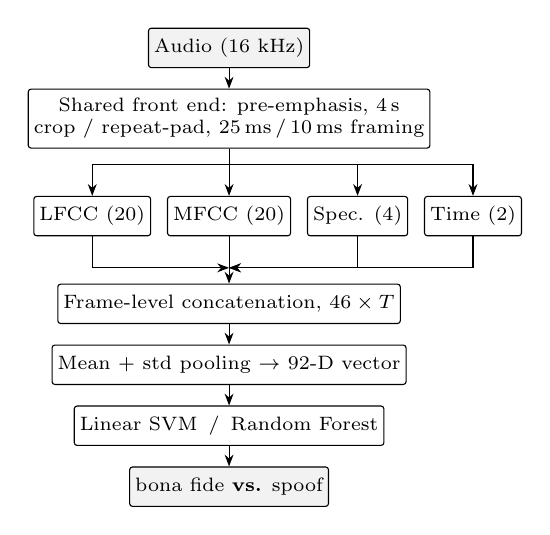
\begin{tikzpicture}[
  node distance=2.6mm,
  box/.style={draw,rounded corners=1pt,align=center,font=\scriptsize,
              minimum height=5mm,inner xsep=2pt},
  >={Stealth[length=1.5mm]}]
\node[box,fill=black!5] (in)  {Audio (16~kHz)};
\node[box,below=of in]  (pre) {Shared front end: pre-emphasis, 4\,s\\crop / repeat-pad, 25\,ms\,/\,10\,ms framing};
\node[box,below=6mm of pre] (mf) {MFCC (20)};
\node[box,left=2mm of mf]   (lf) {LFCC (20)};
\node[box,right=2mm of mf]  (sp) {Spec. (4)};
\node[box,right=2mm of sp]  (td) {Time (2)};
\node[box,below=6mm of mf]  (cat) {Frame-level concatenation, $46 \times T$};
\node[box,below=of cat]  (pool) {Mean $+$ std pooling $\rightarrow$ 92-D vector};
\node[box,below=of pool] (clf)  {Linear SVM \,/\, Random Forest};
\node[box,below=of clf,fill=black!5] (out) {bona fide \textbf{vs.} spoof};
\draw[->] (in) -- (pre);
\draw[->] (pre.south) -- ++(0,-2mm) -| (lf);
\draw[->] (pre.south) -- ++(0,-2mm) -| (mf);
\draw[->] (pre.south) -- ++(0,-2mm) -| (sp);
\draw[->] (pre.south) -- ++(0,-2mm) -| (td);
\draw[->] (lf.south) |- ($(cat.north)+(0,2mm)$);
\draw[->] (mf) -- (cat);
\draw[->] (sp.south) |- ($(cat.north)+(0,2mm)$);
\draw[->] (td.south) |- ($(cat.north)+(0,2mm)$);
\draw[->] (cat) -- (pool);
\draw[->] (pool) -- (clf);
\draw[->] (clf) -- (out);
\end{tikzpicture}
\caption{Detection pipeline. All four feature families share one
preprocessing front end, so comparisons between them are fair.}
\label{fig:pipeline}
\end{figure}

\subsection{Audio Front End}
Signals are resampled to $f_s = 16$~kHz, converted to mono and
pre-emphasised,
\begin{equation}
y[n] = x[n] - \alpha\,x[n-1], \qquad \alpha = 0.97 ,
\end{equation}
then fixed to $4$~s ($64{,}000$ samples) by a deterministic head crop, or by
\emph{repeat}-padding when shorter. Repeat-padding is used instead of
zero-padding so that short files do not acquire an artificial silence cue.
Short-time analysis uses a $25$~ms Hamming window ($N = 400$) with a $10$~ms
hop ($H = 160$) and $n_{\mathrm{FFT}} = 512$:
\begin{equation}
X[k,m] = \sum_{n=0}^{N-1} y[n + mH]\,w[n]\,e^{-j 2\pi k n / n_{\mathrm{FFT}}} .
\end{equation}

Two preprocessing options are deliberately \emph{disabled} by default.
Silence is not trimmed, because leading and trailing silence is a known
database-specific shortcut in ASVspoof; and peak normalisation is off,
because absolute level reflects the source database rather than the
synthesiser. Both remain available as ablations.

\subsection{Cepstral Features}
MFCCs use $20$ coefficients over a mel filter bank,
$m(f) = 2595 \log_{10}(1 + f/700)$. LFCCs follow the same chain but with
$M = 40$ triangular filters spaced \emph{linearly} between $0$ and $f_s/2$:
\begin{equation}
E[i,m] = \sum_{k} H_i[k]\,\bigl|X[k,m]\bigr|^{2} ,
\end{equation}
\begin{equation}
c[q,m] = \sum_{i=1}^{M} \log\bigl(E[i,m]\bigr)
         \cos\!\left[\frac{\pi q\,(i-0.5)}{M}\right] ,
\end{equation}
keeping $q = 1,\dots,20$. The only difference between the two front ends is
the filter spacing, which isolates the effect of high-frequency resolution.

\subsection{Spectral and Time-Domain Descriptors}
Four spectral descriptors are computed per frame. With normalised magnitude
$p[k,m] = |X[k,m]| / \sum_k |X[k,m]|$ and bin frequency $f_k$,
\begin{align}
\mathrm{SC}[m] &= \sum_k f_k\,p[k,m] , \\
\mathrm{SB}[m] &= \Bigl(\textstyle\sum_k (f_k - \mathrm{SC}[m])^{2}\,p[k,m]\Bigr)^{1/2} ,
\end{align}
the roll-off $\mathrm{SR}[m]$ is the smallest $f_{k^\star}$ for which
$\sum_{k \le k^\star} p[k,m] \ge 0.85$, and the flux is
\begin{equation}
\mathrm{SF}[m] = \Bigl(\textstyle\sum_k \bigl(p[k,m] - p[k,m-1]\bigr)^{2}\Bigr)^{1/2} .
\end{equation}
Two time-domain descriptors complete the set: short-time energy
$\mathrm{STE}[m] = \frac{1}{N}\sum_n (y[n+mH]\,w[n])^{2}$ and the
zero-crossing rate
$\mathrm{ZCR}[m] = \frac{1}{2N}\sum_n \bigl|\mathrm{sgn}(y[n{+}1]) - \mathrm{sgn}(y[n])\bigr|$.

\subsection{Pooling and Classification}
Concatenation gives a $46 \times T$ frame-level matrix whose length $T$
varies with the recording. Because classical classifiers need fixed-length
inputs, each feature $d$ is pooled over time,
\begin{equation}
\mu_d = \frac{1}{T}\sum_{m=1}^{T} v_d[m], \qquad
\sigma_d = \sqrt{\frac{1}{T}\sum_{m=1}^{T}\bigl(v_d[m]-\mu_d\bigr)^{2}} ,
\end{equation}
producing a $46 \times 2 = 92$-dimensional utterance vector whose components
keep interpretable names such as \texttt{lfcc\_07\_std}.

Two classifiers are used. The first is a \texttt{StandardScaler} followed by
a linear SVM ($C = 1$, balanced class weights, $10^{4}$ iterations), whose
decision function $f(\mathbf{x}) = \mathbf{w}^{\top}\mathbf{x} + b$ serves
directly as the spoof score. The second is a random forest ($200$ trees,
balanced class weights) scored by its spoof-class probability. Balanced
class weights are essential because the corpus is approximately $90\%$
spoof.

\subsection{Evaluation Metrics}
Besides accuracy, precision, recall and $F_1$, the two metrics that matter
for anti-spoofing are ROC--AUC and the equal error rate, the operating point
at which false-acceptance and false-rejection rates coincide:
\begin{equation}
\mathrm{EER} = \mathrm{FPR}(\tau^\star) = \mathrm{FNR}(\tau^\star), \quad
\tau^\star = \arg\min_{\tau} \bigl|\mathrm{FPR}(\tau) - \mathrm{FNR}(\tau)\bigr| .
\end{equation}
AUC and EER are threshold-independent; reporting them alongside accuracy is
what makes the calibration failure of Section~\ref{sec:calib} visible at all.

%-----------------------------------------------------------------------
% 6. EXPERIMENTS AND RESULTS
%-----------------------------------------------------------------------
\section{Experiments and Results}
\label{sec:results}

\subsection{Data and Protocol}
Table~\ref{tab:data} summarises the data. Training uses the ASVspoof~2019 LA
training partition, from which a $15\%$ speaker-disjoint validation split is
carved out so that no speaker appears in both. The manifest builder
additionally rejects duplicated utterance identifiers, speakers crossing
incompatible splits, and byte-identical audio across splits. A
quality-control pass over $2{,}000$ sampled files confirmed a uniform
$16$~kHz rate, no unreadable files, a mean level near $-19$~dBFS and
negligible clipping ($<5 \times 10^{-5}$).

Three test conditions of increasing difficulty are used. (i) The matched
validation split. (ii) The LA evaluation set: $71{,}237$ utterances from
$67$ unseen speakers generated by thirteen attacks (A07--A19) absent from
training. (iii) A class-balanced $11{,}070$-utterance subset of
ASVspoof~2021 DF---a different corpus with different codecs and generators.
Models are never retrained between conditions.

\begin{table}[!t]
\caption{Data partitions (ASVspoof 2019 LA; DF subset from ASVspoof 2021).}
\label{tab:data}
\centering
\footnotesize
\begin{tabular}{lrrrl}
\toprule
Partition & Utterances & Speakers & Spoof \% & Role \\
\midrule
Train      & 21{,}521 & 17 & 89.8 & model fitting \\
Validation &  3{,}859 &  3 & 89.9 & speaker-disjoint tuning \\
LA eval    & 71{,}237 & 67 & 89.7 & unseen attacks A07--A19 \\
DF subset  & 11{,}070 & --- & 50.0 & cross-corpus test \\
\bottomrule
\end{tabular}
\end{table}

\subsection{In-Domain Results}
Table~\ref{tab:val} reports matched-condition results for all eight
model/feature combinations. Three observations stand out. First, LFCC
clearly beats MFCC: for the SVM the EER falls from $23.32\%$ to $12.82\%$,
confirming that the linearly spaced filter bank retains high-frequency
artefacts that the mel scale discards. Second, adding the six spectral and
time-domain descriptors to MFCC helps but does not close the gap
($17.96\%$ EER). Third, the full $92$-dimensional vector is best: the linear
SVM reaches $97.59\%$ accuracy, $0.9867$ $F_1$, $0.9919$ AUC and a $4.35\%$
EER. Traditional features are therefore far from useless---under matched
conditions they support a competent detector.

\begin{table}[!t]
\caption{Matched-condition results on the speaker-disjoint validation split.}
\label{tab:val}
\centering
\footnotesize
\begin{tabular}{llccccc}
\toprule
Model & Features & Dim & Acc. & $F_1$ & AUC & EER \\
\midrule
SVM & MFCC       & 40 & 0.816 & 0.891 & 0.862 & 0.2332 \\
RF  & MFCC       & 40 & 0.924 & 0.959 & 0.925 & 0.1521 \\
SVM & LFCC       & 40 & 0.942 & 0.968 & 0.952 & 0.1282 \\
RF  & LFCC       & 40 & 0.934 & 0.965 & 0.972 & 0.0976 \\
SVM & MFCC+Spec. & 46 & 0.881 & 0.932 & 0.905 & 0.1796 \\
RF  & MFCC+Spec. & 46 & 0.924 & 0.960 & 0.917 & 0.1559 \\
\textbf{SVM} & \textbf{Combined} & \textbf{92} & \textbf{0.976}
      & \textbf{0.987} & \textbf{0.992} & \textbf{0.0435} \\
RF  & Combined   & 92 & 0.937 & 0.966 & 0.973 & 0.0837 \\
\bottomrule
\end{tabular}
\end{table}

\subsection{Unseen Attacks and Cross-Corpus Generalisation}
Table~\ref{tab:gen} repeats the evaluation on the LA evaluation set and on
the DF subset. The best result on unseen attacks is the random forest with
combined features, at $89.15\%$ accuracy and $12.84\%$ EER---a moderate and
expected degradation. On DF, however, \emph{every} configuration collapses
into the $30.5$--$38.1\%$ EER band, with AUC falling by $0.12$ to $0.22$
relative to the LA evaluation set. A detector trained on 2019 LA does not
transfer to 2021 DF, reproducing the conclusion of~\cite{muller2022} with
classical features.

\begin{table}[!t]
\caption{Generalisation: identical trained models, harder test conditions.}
\label{tab:gen}
\centering
\footnotesize
\begin{tabular}{llcccc}
\toprule
& & \multicolumn{2}{c}{LA eval (unseen attacks)}
  & \multicolumn{2}{c}{DF (cross-corpus)} \\
\cmidrule(lr){3-4}\cmidrule(lr){5-6}
Model & Features & AUC & EER & AUC & EER \\
\midrule
SVM & MFCC       & 0.865 & 0.2137 & 0.719 & 0.3379 \\
RF  & MFCC       & 0.893 & 0.1753 & 0.772 & 0.3051 \\
SVM & LFCC       & 0.808 & 0.2668 & 0.653 & 0.3808 \\
RF  & LFCC       & 0.918 & 0.1549 & 0.697 & 0.3674 \\
SVM & MFCC+Spec. & 0.895 & 0.1828 & 0.731 & 0.3252 \\
RF  & MFCC+Spec. & 0.919 & 0.1563 & 0.754 & 0.3208 \\
SVM & Combined   & 0.861 & 0.2181 & 0.704 & 0.3396 \\
\textbf{RF} & \textbf{Combined} & \textbf{0.939} & \textbf{0.1284}
      & 0.742 & 0.3450 \\
\bottomrule
\end{tabular}
\end{table}

\subsection{Qualitative Analysis: A Calibration Failure, Not a Feature Failure}
\label{sec:calib}
The most instructive result is the behaviour of the best validation model.
Retrained on train\,$+$\,validation ($25{,}380$ utterances) and applied to
the $71{,}237$-utterance LA evaluation set, the linear SVM on combined
features scores only $57.81\%$ accuracy and $0.693$ $F_1$---yet its AUC is
$0.8615$ and its EER is $21.81\%$. The confusion matrix in
Fig.~\ref{fig:cm} shows why: precision is $0.996$ while recall is $0.532$.
Almost every utterance the model calls spoof really is spoof, but it misses
nearly half of them. The ROC curve in Fig.~\ref{fig:roc} lies well above the
diagonal, so the \emph{ranking} of utterances remains informative.

The fixed decision boundary $f(\mathbf{x}) = 0$ learned on the six training
attacks simply sits in the wrong place for the thirteen evaluation attacks,
whose scores shift toward the bona fide side; the EER threshold for the same
model is $-2.45$, not $0$. This distinguishes two failure modes that a
single accuracy number would conflate: the features still separate the
classes, but the operating point does not survive the shift. It also
explains why the random forest---whose probability outputs are bounded in
$[0,1]$ and therefore shift far less---generalises better despite being the
weaker in-domain model. The practical lesson is that a countermeasure must
be calibrated on data resembling deployment, and must be reported with
threshold-free metrics.

\begin{figure}[!t]
\centering
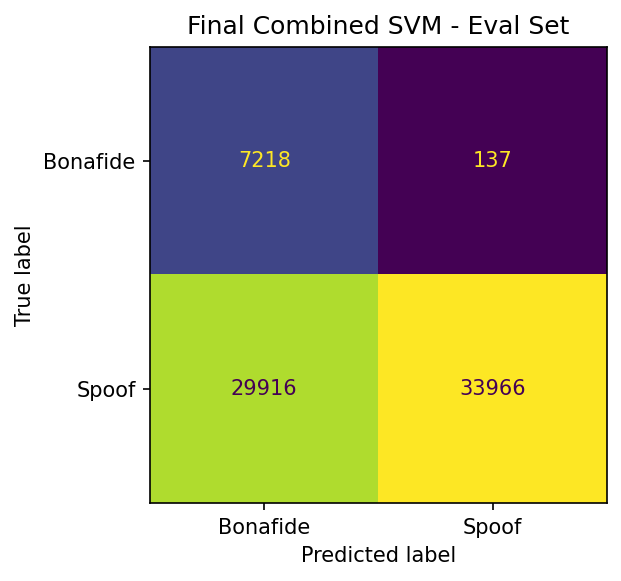
\includegraphics[width=0.74\columnwidth]{final_confusion_matrix.png}
\caption{Confusion matrix of the final linear SVM (combined features) on the
71{,}237-utterance LA evaluation set. High precision with low recall: the
threshold, not the feature space, is misplaced.}
\label{fig:cm}
\end{figure}

\begin{figure}[!t]
\centering
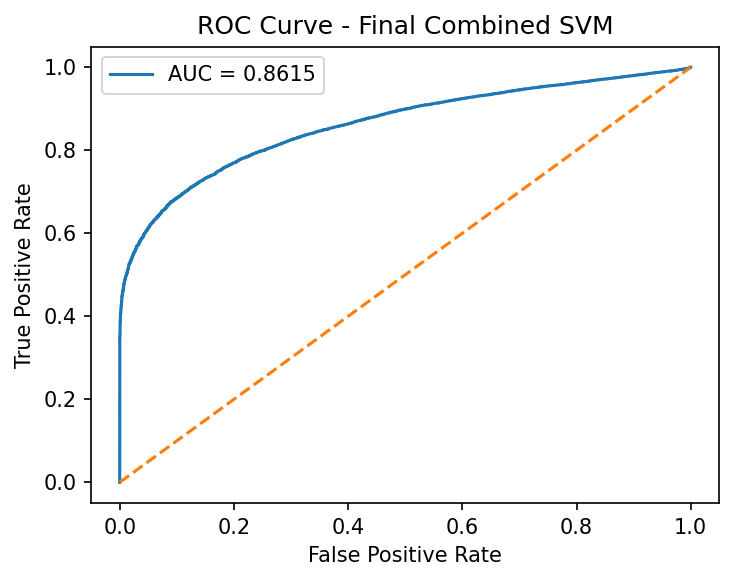
\includegraphics[width=0.82\columnwidth]{final_roc_curve.png}
\caption{ROC curve of the same model (AUC $= 0.861$, EER $= 21.8\%$). The
ranking stays informative even where accuracy is close to chance.}
\label{fig:roc}
\end{figure}

\subsection{Live Demonstration}
The trained pipeline was packaged as an interactive script
(\texttt{06\_live\_demo.py}) that loads the serialised SVM, runs a single
recording through the identical preprocessing and feature code used in
training, and prints the decision together with its margin. Reusing the
training-time extraction functions rather than reimplementing them
guarantees that no train/inference skew is introduced.

%-----------------------------------------------------------------------
% 7. TEAM MEMBER CONTRIBUTION
%-----------------------------------------------------------------------
\section{Team Member Contribution}
\textbf{Tala Hussary (Phase~1 --- data foundation).} Designed
\texttt{config.yaml} and the configuration loader; implemented the shared
audio front end (\texttt{src/audio.py}: resampling, pre-emphasis,
crop/repeat-pad, framing); wrote the manifest builder and the
speaker-disjoint splitter with duplicate- and leakage-detection
(\texttt{src/manifest.py}); implemented the quality-control pass and its
figures (\texttt{src/qc.py}); authored \texttt{tests/test\_phase1.py} and the
dataset documentation.

\textbf{Donia Said (Phase~2A --- feature extraction).} Implemented all
feature extractors in \texttt{src/features.py}: MFCC, the linear triangular
filter bank and DCT for LFCC, the four spectral descriptors, short-time
energy and zero-crossing rate; implemented frame-level concatenation,
mean/standard-deviation pooling and the feature-naming scheme; wrote the
batch extraction script (\texttt{02\_extract\_features.py}) and the
eight-case unit-test suite (\texttt{tests/test\_features.py}); authored the
methodology equations in this report.

\textbf{Malak Obaid (Phases~2B and 3 --- modelling and evaluation).}
Implemented the classical training and comparison script over the four
feature sets (\texttt{03\_train\_classical.py}), the EER routine and all
metric reporting; ran the final evaluation on the LA evaluation set
(\texttt{04\_final\_evaluation.py}), the all-model sweep
(\texttt{05\_eval\_all\_models.py}) and the ASVspoof~2021~DF cross-corpus
experiment (\texttt{07}--\texttt{09}); produced the confusion matrices and
ROC figures; built the live demo; performed the calibration analysis and
prepared the presentation.

All three members jointly reviewed the code, verified every number reported
here against the generated CSV files in \texttt{reports/}, and edited this
manuscript.

%-----------------------------------------------------------------------
% 8. CONCLUSION
%-----------------------------------------------------------------------
\section{Conclusion}
The objective was to determine whether traditional speech features can
detect AI-generated speech, and it was met. A complete, reproducible
pipeline was built from raw corpora to a live demonstrator, and eight
model/feature configurations were measured under three conditions of
increasing difficulty.

The main findings are as follows. (i) Classical features are genuinely
informative: a linear SVM on $92$ pooled MFCC, LFCC, spectral and
time-domain statistics reaches $4.35\%$ EER in matched conditions.
(ii) LFCC consistently outperforms MFCC, supporting the view that synthesis
artefacts live in the high band that the mel scale compresses.
(iii) Performance degrades gracefully on unseen attacks (best $12.84\%$ EER)
but severely across corpora ($\ge 30.5\%$ EER). (iv) The sharp accuracy drop
of the best in-domain model is a threshold-calibration failure rather than a
representation failure---a distinction visible only because AUC and EER were
reported alongside accuracy.

The main limitations are that pooling to means and standard deviations
discards all temporal structure, that a linear SVM cannot model interactions
between feature families, that only two corpora were used, and that the
cross-corpus test used a single balanced partition of the DF evaluation set.
Future work should add delta and delta-delta coefficients, score
normalisation or per-domain threshold calibration, the constant-Q cepstral
front end used by the ASVspoof baselines, the planned spectrogram CNN as a
learned-feature contrast, and the WaveFake corpus to separate
\emph{generator} shift from \emph{channel} shift. The broader lesson is that
a countermeasure is only characterised once it has been tested outside the
corpus it was trained on.

%-----------------------------------------------------------------------
% AI DISCLOSURE + REFERENCES
%-----------------------------------------------------------------------
\section*{Acknowledgment and AI-Tool Disclosure}
The use of AI assistants is permitted by the project specification and is
disclosed here. \emph{Claude} (Anthropic)~\cite{claude} assisted with
Phase~1 code generation, docstring and documentation drafting, test design,
and \LaTeX{} writing support for this report. \emph{ChatGPT}
(OpenAI)~\cite{chatgpt} assisted with implementation and debugging of the
feature-extraction pipeline and its unit tests. No AI tool produced any
experimental result: all numbers reported here were generated by executing
the project code, and every AI-suggested line was reviewed, run and tested
by the authors.

\begin{thebibliography}{99}
\bibitem{todisco2019}
M. Todisco \emph{et al.}, ``ASVspoof 2019: Future horizons in spoofed and
fake audio detection,'' in \emph{Proc. Interspeech}, Graz, Austria, 2019,
pp. 1008--1012.

\bibitem{yamagishi2021}
J. Yamagishi \emph{et al.}, ``ASVspoof 2021: Accelerating progress in
spoofed and deepfake speech detection,'' in \emph{Proc. ASVspoof Challenge
Workshop}, 2021, pp. 47--54.

\bibitem{frank2021}
J. Frank and L. Sch\"onherr, ``WaveFake: A data set to facilitate audio
deepfake detection,'' in \emph{Proc. NeurIPS Datasets and Benchmarks
Track}, 2021.

\bibitem{muller2022}
N. M\"uller, P. Czempin, F. Dieckmann, A. Froghyar, and K. B\"ottinger,
``Does audio deepfake detection generalize?'' in \emph{Proc. Interspeech},
Incheon, Korea, 2022, pp. 2783--2787.

\bibitem{sahidullah2015}
M. Sahidullah, T. Kinnunen, and C. Hanil\c{c}i, ``A comparison of features
for synthetic speech detection,'' in \emph{Proc. Interspeech}, Dresden,
Germany, 2015, pp. 2087--2091.

\bibitem{davis1980}
S. Davis and P. Mermelstein, ``Comparison of parametric representations for
monosyllabic word recognition in continuously spoken sentences,''
\emph{IEEE Trans. Acoust., Speech, Signal Process.}, vol. 28, no. 4,
pp. 357--366, Aug. 1980.

\bibitem{mcfee2015}
B. McFee \emph{et al.}, ``librosa: Audio and music signal analysis in
Python,'' in \emph{Proc. 14th Python in Science Conf. (SciPy)}, 2015,
pp. 18--25.

\bibitem{pedregosa2011}
F. Pedregosa \emph{et al.}, ``Scikit-learn: Machine learning in Python,''
\emph{J. Mach. Learn. Res.}, vol. 12, pp. 2825--2830, 2011.

\bibitem{harris2020}
C. R. Harris \emph{et al.}, ``Array programming with NumPy,''
\emph{Nature}, vol. 585, pp. 357--362, 2020.

\bibitem{virtanen2020}
P. Virtanen \emph{et al.}, ``SciPy 1.0: Fundamental algorithms for
scientific computing in Python,'' \emph{Nature Methods}, vol. 17,
pp. 261--272, 2020.

\bibitem{claude}
Anthropic, ``Claude,'' large language model assistant, 2026. [Online].
Available: \url{https://claude.ai}

\bibitem{chatgpt}
OpenAI, ``ChatGPT,'' large language model assistant, 2026. [Online].
Available: \url{https://chat.openai.com}
\end{thebibliography}

\end{document}
